\documentclass[journal]{IEEEtran}
\usepackage[UTF8,scheme=plain,fontset=fandol]{ctex}
\usepackage{amsmath,amsfonts,amssymb}
\usepackage{algorithmic}
\usepackage{algorithm}
\usepackage{array}
\usepackage[caption=false,font=normalsize,labelfont=sf,textfont=sf]{subfig}
\usepackage{textcomp}
\usepackage{stfloats}
\usepackage{url}
\usepackage{verbatim}
\usepackage{graphicx}
\usepackage{cite}
\usepackage{bm}
\usepackage{multirow}
\usepackage{balance}

\newtheorem{proposition}{命题}
\newtheorem{theorem}{定理}
\renewcommand{\abstractname}{摘\quad 要}
\renewcommand{\IEEEkeywordsname}{关键词}
\floatname{algorithm}{算法}

\renewcommand{\topfraction}{0.95}
\renewcommand{\bottomfraction}{0.5}
\renewcommand{\textfraction}{0.05}
\renewcommand{\floatpagefraction}{0.60}
\setcounter{topnumber}{4}
\setcounter{totalnumber}{6}

% ---- 紧凑的公式与浮动体间距（控制页数） ----
\setlength{\abovedisplayskip}{4pt plus 1pt minus 1pt}
\setlength{\belowdisplayskip}{4pt plus 1pt minus 1pt}
\setlength{\abovedisplayshortskip}{2pt plus 1pt}
\setlength{\belowdisplayshortskip}{2pt plus 1pt}
\setlength{\jot}{2pt}
\setlength{\textfloatsep}{7pt plus 2pt minus 2pt}
\setlength{\floatsep}{6pt plus 2pt minus 2pt}
\setlength{\intextsep}{6pt plus 2pt minus 2pt}
\setlength{\dbltextfloatsep}{7pt plus 2pt minus 2pt}
\setlength{\dblfloatsep}{6pt plus 2pt minus 2pt}

\begin{document}

\title{时变信道下面向V2X风险理解的\\语用感知Token调度}

\author{Changyu~Zhang, Lingyun~Lu, Wei~Ni,~\IEEEmembership{Senior Member,~IEEE}, Xiaoqiang~Zhu,~\IEEEmembership{Member,~IEEE}
\thanks{Changyu~Zhang和Lingyun~Lu均来自北京交通大学软件学院，北京100044（电子邮箱：25121368@bjtu.edu.cn；lylu@bjtu.edu.cn）。通信作者：Changyu~Zhang。}
\thanks{Wei~Ni来自Edith Cowan University工程学院，Perth, WA 6027, Australia（电子邮箱：wei.ni@ieee.org）。}
\thanks{Xiaoqiang~Zhu来自北京交通大学网络空间安全学院，北京100044（电子邮箱：xqzhu@bjtu.edu.cn）。}}

\markboth{IEEE Transactions on Vehicular Technology}%
{Zhang and Lu: 面向V2X风险理解的Token级语义传输}

\maketitle

\begin{abstract}
城市路口在视距受阻时，单车视角不足以完成风险理解，需要车辆经车联网上行把感知信息送至路侧单元（RSU），由RSU依据接收的语义报告完成风险相关问答，且必须在有限频谱与高移动性下控制通信开销并保障传输可靠性；这类风险理解只依赖画面中少数与冲突相关的语义要素。若仍无差别地上传原始图像或完整感知数据，开销将随内容规模增长而逼近带宽极限，与任务真正需要的信息量严重失配。生成式语义通信（GSC）沿传输任务语义而非原始比特的思路，由视觉语言模型把多模态输入压缩为紧凑的提示序列，可把传输开销降低一至两个数量级；但提示序列中不同Token对任务的贡献并不相同，其重要性还随瞬时信道状态变化。本文提出语用感知的Token级选择与调度方法。该方法融合因果自注意力结构重要度、语义方向一致性与删除感知梯度敏感度构造统一语用度量，并引入保持因果方向的语义耦合模型，使效用由实际成功接收的Token集合决定；在不完美信道状态信息（CSI）下以条件解码概率刻画接收可靠性、以可靠信道容量给出等效比特预算，并将Token选择与编码保护联合优化。求解时先用拉格朗日方法处理线性松弛，再由具有理论保证的极点舍入得到可行解，并以耦合感知局部改进提升效用；多终端场景以在线语义价格实现比例公平带宽分配。理论分析给出语义代理误差、传输速率与VQA精度之间的可证边界，并把端到端差距分解为优化误差、语义代理误差、模型失配与信道中断四项。在V2X-QA上、满足端侧（车载终端）算力小于边侧（路侧协调器）这一部署前提的主线配置（端侧4B$\rightarrow$边侧8B）下，所提方法与最强已发表基线精度统计不可区分（$1080$组配对$46{:}43$，$p=0.83$），并取得全部可部署方法中最高的资源效率（较精度最强的可部署基线\textbf{相对}提升$47.9\%$，绝对高出$15.8$~acc/kSym）、传输符号开销降低约$32\%$。
\end{abstract}

\begin{IEEEkeywords}
任务导向语义通信；V2X风险理解；Token级语义传输；生成式语义通信；语义耦合；时变信道调度
\end{IEEEkeywords}

\section{引言}

在城市路口和视距受阻（non-line-of-sight，NLOS）场景中，单车视角难以覆盖被遮挡的交通参与者，车辆因而需要经车联网上行把任务相关感知信息发送至路侧单元（road side unit，RSU），由RSU依据接收的语义报告完成风险相关问答。该过程同时受到频谱稀缺、高移动性和时变衰落的约束，需要在有限资源下保障任务相关信息的可靠交付。与原始图像包含的大量像素不同，风险理解往往只依赖目标位置、速度、运动方向等少数冲突相关要素；无差别上传完整图像或高维特征会使通信开销与任务真正需要的信息量严重失配。

任务导向语义通信通过传输与下游决策有关的信息而非逐比特复现信源，为消除上述失配提供了新的设计范式~\cite{gunduz2023beyond}。早期方案主要依靠深度联合信源信道编码（DeepJSCC）在无线信道上直接传输紧凑特征~\cite{bourtsoulatze2019deep,xie2021task}。随着视觉语言模型（VLM）和大语言模型（LLM）的发展，生成式语义通信进一步把多模态内容表示为自然语言提示序列，仅传输足以支持接收端推理的文本语义~\cite{Qiao2024latency,ren2025generative}。近期Token通信框架则把Transformer原生Token提升为通信单元，使模型内部表示与无线传输粒度能够直接衔接~\cite{qiao2025tokcom}。

然而，从“传输整条提示”推进到“选择并可靠传输部分Token”仍有三项不足。\textbf{不足（1）语用效用建模。}单一注意力、困惑度或删除代理难以同时反映因果结构、任务语义方向和删除损失，独立分数相加还会忽略剪枝后的集合交互。\textbf{不足（2）信道与语义联合决策。}不完美CSI下的解码概率和保护开销会共同改变Token价值，分开决定Token集合与保护模式无法充分利用可靠预算并控制残余错误。\textbf{不足（3）多终端语义公平与跨层解释。}按物理速率或固定比例分配带宽忽略各终端的边际语义收益，且缺少从可靠预算、Token保留率到任务错误的分析联系。第~\ref{sec:related}节进一步梳理这些不足。

为此，本文提出面向V2X风险理解的语用感知Token选择与调度框架：以多维语用度量和因果集合效用解决不足（1），以Token--保护模式联合优化解决不足（2），以在线语义价格和跨层性能界解决不足（3），从而统一语义选择、可靠传输与多终端资源调度。



本文的主要贡献概括如下。
\begin{itemize}
\item \textbf{针对不足（1）}，提出融合因果自注意力结构重要度、语义方向一致性与删除感知梯度敏感度的Token语用度量，并构造保持因果方向的集合耦合模型，使效用只由实际成功接收的Token及其有效上下文决定，从目标函数层面消除未选Token的效用泄漏。
\item \textbf{针对不足（2）}，在不完美CSI下统一建模Token选择、差异化保护和残余解码错误。所形成的二次多选择背包问题先由拉格朗日断点搜索求解线性松弛，再经具有$1/2$基础保证的LP极点舍入与耦合感知局部改进得到可行解；在精度与最强可部署基线统计不可区分时，资源效率相对提高$47.9\%$、符号开销降低约$32\%$。
\item \textbf{针对不足（3）}，构建基于在线语义价格的多车辆比例公平调度机制，并建立从可靠传输预算、Token保留率到VQA错误上界的分析链条；端到端性能差距被分解为优化、语义代理、模型失配和信道中断四项。
\end{itemize}

全文共分六节。第~\ref{sec:related}节回顾相关工作；第~\ref{sec:system}节给出V2X架构、任务与信道模型；第~\ref{sec:utility}节提出语用感知Token选择与调度方法并分析其性能；第~\ref{sec:exp}节给出实验验证；第~\ref{sec:conclusion}节总结全文。

\section{相关工作}
\label{sec:related}

\subsection{V2X任务导向语义通信}

语义通信把通信质量由比特恢复精度推进到语义或任务效用~\cite{gunduz2023beyond,xie2021deep}，在视觉问答等多用户任务中可直接围绕推理准确率设计传输表示~\cite{xie2021task}。面向车联网，TCMSC将语义频谱效率、功耗和时延违约概率纳入多业务车辆调度~\cite{yuan2025tcmsc}；基于接收端上下文的相关性选择进一步说明，V2X消息中只有一部分内容会改变目标车辆的感知或决策~\cite{lusvarghi2026relevance}。协同感知研究也从模拟特征传输转向可兼容数字V2X链路的任务语义编码，以缓解低信噪比下的悬崖效应~\cite{gan2026cods}。这些工作证明了内容选择对于V2X扩展性的重要性，但多数仍在对象、特征图或整条消息层面度量语义价值，尚未处理自然语言报告内部Token之间的细粒度差异及上下文依赖。

\subsection{生成式语义通信与Token选择}

生成式语义通信利用生成模型的先验知识，以低码率条件信息替代高维信源的逐样本复现~\cite{erdemir2023generative,Qiao2024latency}。预训练VLM能够先把图像转写为文本报告，再由边缘LLM完成任务推理，从而形成适于设备--边缘协同的提示传输路径~\cite{ren2025generative,jiang2025large}。TokCom进一步以Token作为模型和网络共享的基本单元，并利用跨模态上下文恢复丢失内容~\cite{qiao2025tokcom}。另一方面，LLMLingua、LongLLMLingua和LLMLingua-2分别以困惑度、长上下文重排和蒸馏分类器压缩提示~\cite{jiang2023llmlingua,jiang2024longllmlingua,pan2024llmlingua2}；Selective-Context与EFPC也从冗余过滤和任务自适应分类角度减少输入长度~\cite{li2023selective,cao2025efpc}。上述提示压缩方法主要面向推理成本，在无差错上下文上决定保留内容，因而没有显式描述无线擦除、保护模式和剪枝后Token集合价值之间的耦合。

\subsection{信道感知语义资源分配}

信息瓶颈为任务相关表示学习提供了统一准则~\cite{shao2021learning}；面向衰落信道的OFDM引导DeepJSCC和在线自适应变换编码增强了语义传输对信道变化的适应能力~\cite{Yang2022ofdm,daiTowardAdaptive}。网络层研究已联合优化用户关联与带宽~\cite{xia2023joint}，并开始讨论大模型驱动的多用户生成式语义通信~\cite{yang2025rethinking}。然而，现有方案通常把语义压缩率或整条消息效用作为资源分配输入，难以同时回答三个问题：剪枝后Token集合的真实价值、给定Token应采用何种保护模式，以及带宽应如何依据车辆的边际语义收益分配。本文以因果集合效用、条件解码概率和在线语义价格统一这三个层次。

\section{系统模型}
\label{sec:system}

\subsection{V2X架构与任务模型}

\begin{figure*}[t]
\centering
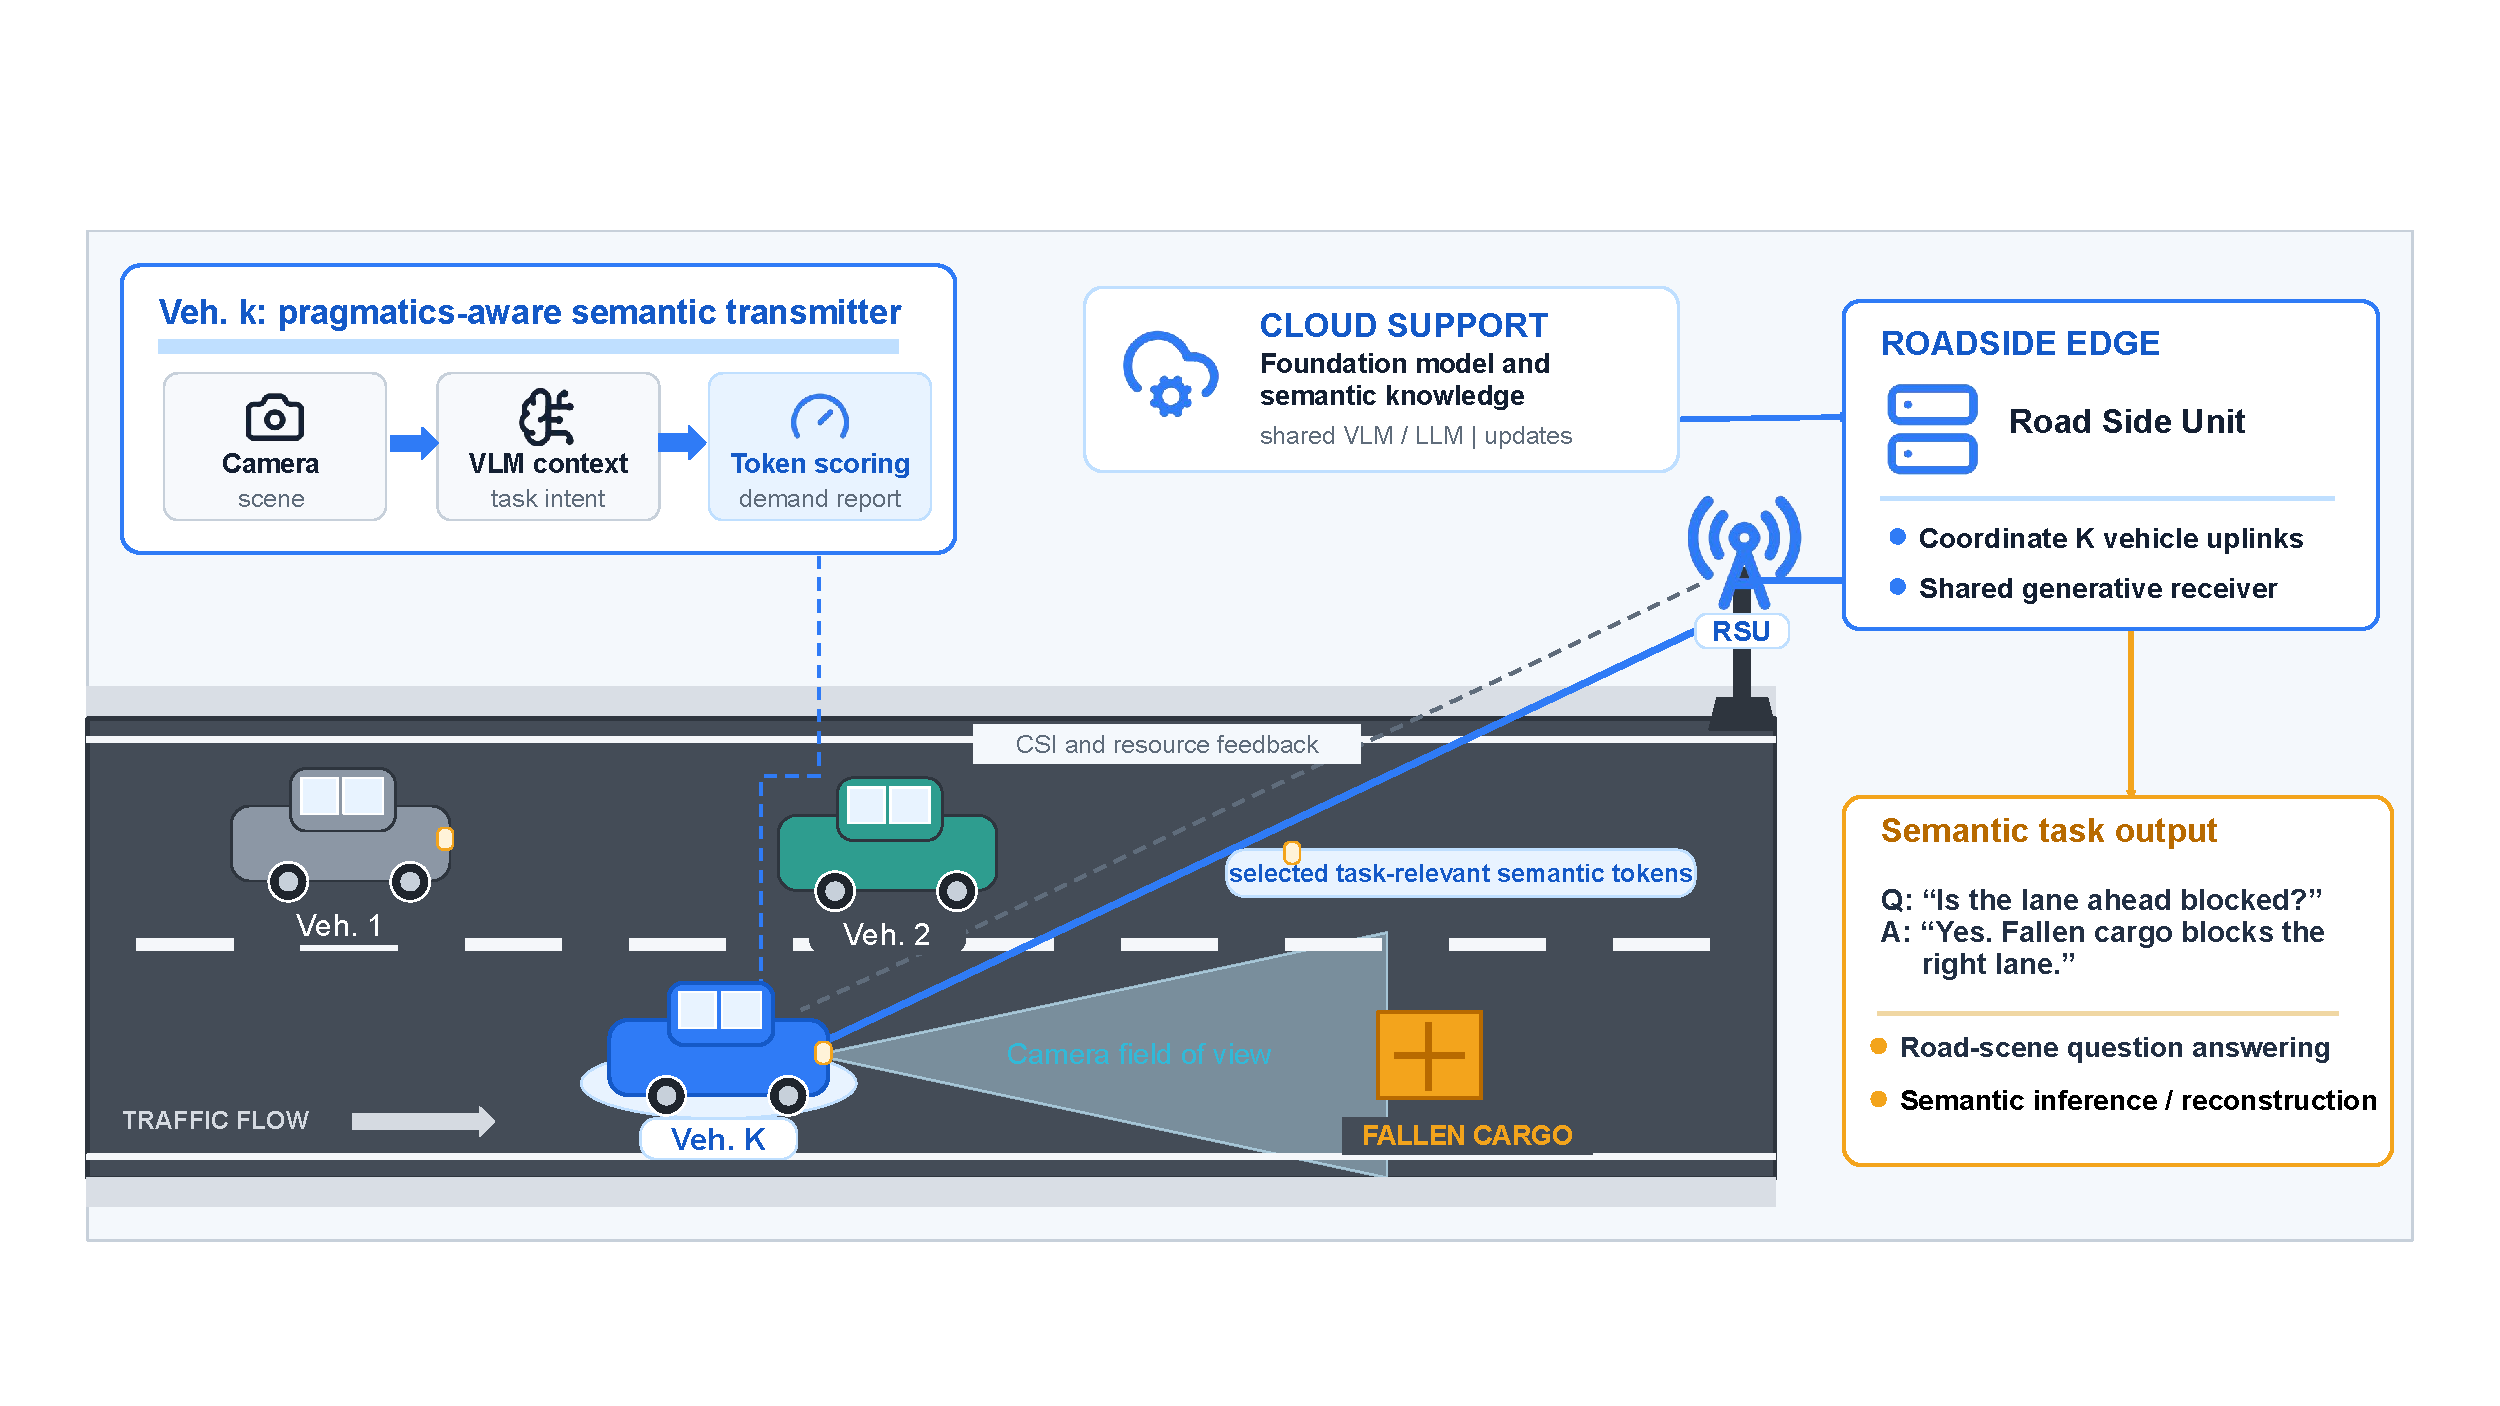
\includegraphics[width=0.72\textwidth,trim=0 32 0 40,clip]{images/vehicular_application_scenario.pdf}
\caption{共享上行GSC系统的V2X部署。车辆在本地完成语义提取和语用评分，仅向RSU上报紧凑的语义需求；RSU协调$K$辆车的上行资源并下发授权，车辆随后确定Token集合及保护模式。车辆上传经过选择与保护编码的报告Token，RSU解码后完成风险相关问答；云端仅在较慢时间尺度上更新基础模型和语义知识。}
\label{fig:vehicular_scenario}
\end{figure*}

\begin{figure*}[t]
\centering
\includegraphics[width=0.72\textwidth]{images/gsc_architecture.pdf}
\caption{多终端语用感知GSC架构及Token贡献评估流程。每个终端完成VLM编码和本地语用评估后，仅向联合带宽分配器上报紧凑的语义需求标量$p_k$。协调器将该报告与CSI结合，向终端返回可靠资源预算；终端收到授权后，再执行Token剪枝和保护编码，并完成上行语义传输。图中下半部分给出了结构依赖、语义表示和任务损失敏感度的融合过程，以及随后的语义耦合修正。后文以由$\mu_{k,\tau}$导出的边际语义报告实现$p_k$，并以$C_{\tau}^{(k)}$表示分配给终端$k$的可靠资源预算。}
\label{fig:framework}
\end{figure*}

图~\ref{fig:vehicular_scenario}给出部署场景，图~\ref{fig:framework}进一步展开语义处理与资源协调流程。本文考虑$K$个终端共享同一个上行接收端；在车联网实例中，一个终端即一辆车，上行接收端即RSU。为叙述简洁，下文把第$k$辆车记为终端$k$，把RSU记为接收端（在涉及多终端协调时亦称协调器），并在实验部分按模型所处位置分别称为端侧与边侧。本文研究从车辆报告生成、Token选择与保护、上行传输到RSU任务推理的语义通信链路，输出为风险相关问题的答案。多终端共享上行资源，跨车辆目标关联与多视角融合不作为本文的优化与实验验证对象。报告生成、语用评分、调度及接收端推理的计算开销与完整任务响应时间在第~\ref{sec:exp-lat}节分别定义。终端$k$将图像$I_k$、问题$Q_k$及相关上下文转换为提示序列，其中$w_i^{(k)}$为第$i$个Token，$\bm e_i^{(k)}$为其$d$维嵌入
\begin{equation}
\mathcal{P}^{(k)}=\{w_1^{(k)},\ldots,w_{N_k}^{(k)}\},
\qquad
\bm e_i^{(k)}\in\mathbb{R}^{d}.
\label{eq:prompt}
\end{equation}

系统将控制信令与语义数据明确分开传输。各终端先在本地完成VLM推理、语用评分与耦合评估，并据本地语义效用形成标量语义需求报告$p_{k,\tau}$（不上传Token嵌入或候选Token集合），再通过预留的低速率上行控制资源发送。接收端由导频或探测参考信号估计上行CSI（该预配置控制资源不计入语义数据传输预算），综合各终端语义需求与信道状态在$K$个终端间统一分配共享时频资源，并通过下行控制信道返回带宽授权$B_{k,\tau}$及适用的链路模式信息。最后，终端$k$在授权约束下确定Token与保护模式的组合，经调度后的上行数据信道发送保护后的Token载荷，接收端完成信道解码后调用生成式任务模型处理恢复的语义信息，用于答案生成或视觉问答等下游任务。

由此可见，Token的语义重要性及其最终保护模式由掌握Token内容的终端决定，接收端只负责确定终端之间的资源预算并给出可用的链路自适应选项；两类决策相互配合，从而在无须把全部候选Token集中到接收端的前提下实现Token选择、保护编码与跨终端资源分配的联合优化。本文研究多个车辆共享同一RSU的上行资源，收发关联与干扰耦合的多通信对扩展见补充材料。

分别以$\bm\theta_{\mathrm T}^{(k)}$和$\bm\theta_{\mathrm R}$表示发送端代理模型与接收端任务模型的参数。记发送端可用信息为$\mathcal S_{\mathrm T}^{(k)}=\{I_k,Q_k\}$、接收端可用信息为$\mathcal S_{\mathrm R}^{(k)}=\{Q_k\}$，而原始图像$I_k$不参与上行传输。对于目标答案序列$\bm y_k^\star=\{y_{k,1}^\star,\ldots,y_{k,T_y}^\star\}$，模型$m\in\{\mathrm T,\mathrm R\}$对应的自回归负对数似然（NLL）定义为
\begin{equation}
\mathcal L_m^{(k)}(\mathcal P)
=-
\sum_{t=1}^{T_y}
\log p_{\bm\theta_m^{(k)}}
\!\left(
y_{k,t}^\star\mid \bm y_{k,<t}^\star,\mathcal S_m^{(k)},\mathcal P
\right),
\label{eq:task_loss}
\end{equation}
为统一符号起见，记$\bm\theta_{\mathrm R}^{(k)}=\bm\theta_{\mathrm R}$。系统最终关注的是接收端损失$\mathcal L_{\mathrm R}^{(k)}$，但发送端通常无法访问接收端的梯度。因此，本文根据$\mathcal L_{\mathrm T}^{(k)}$构造Token分数，并通过模型失配界建立该分数与接收端任务性能之间的联系。

对于多项选择VQA，若最大概率判决给出了错误答案，则正确答案的概率必然不超过$1/2$。因此，
\begin{equation}
\mathbf 1\{\widehat y_k\neq y_k^\star\}
\leq \frac{\mathcal L_{\mathrm R}^{(k)}}{\log 2},
\qquad
\Pr(\widehat y_k\neq y_k^\star)
\leq \frac{\mathbb E[\mathcal L_{\mathrm R}^{(k)}]}{\log 2}.
\label{eq:vqa_error_bound}
\end{equation}
需要强调的是，本文的理论目标并不是假设梯度范数与VQA准确率之间存在线性关系，而是控制由Token删除与传输失败引起的NLL增量，并据此约束一个具有明确含义的VQA错误概率上界。

\subsection{时变信道与可靠传输}

令$h_{\tau}^{(k)}\in\mathbb C$为时隙$\tau$中终端$k$的信道系数。不完美CSI建模为
\begin{equation}
\widehat h_{\tau}^{(k)}=h_{\tau}^{(k)}+e_{\tau}^{(k)},
\qquad
e_{\tau}^{(k)}\sim\mathcal{CN}(0,\sigma_e^2).
\label{eq:csi}
\end{equation}
信道可采用Rayleigh衰落、Rician衰落、频率选择性衰落或基于射线追踪的统计模型。后续分析并不依赖某一种特定分布，只要求能够获得给定$\widehat h_{\tau}^{(k)}$时$h_{\tau}^{(k)}$的条件分布，或由近期信道观测估计出的保守置信下界。

具有信道边信息时，可达容量取决于信道信息由哪一侧掌握以及估计的准确程度~\cite{goldsmith1997capacity,medard2000imperfect}。若把$\widehat h_{\tau}^{(k)}$直接代入完美CSI条件下的Shannon容量公式，就等同于把信道估计值视为真实值，存在估计误差时会高估可用传输能力。给定允许的中断概率$\varepsilon_{\mathrm{out}}$，本文将条件可靠频谱效率定义为
\begin{align}
c_{\varepsilon}^{(k)}(\widehat h_{\tau}^{(k)})
=\sup\big\{c:~&\Pr[\log_2(1+\bar\gamma|h_{\tau}^{(k)}|^2)\geq c
\mid \widehat h_{\tau}^{(k)}]
\notag\\[-0.2em]
&\geq 1-\varepsilon_{\mathrm{out}}\big\},
\label{eq:reliable_spectral_efficiency}
\end{align}
其中，$\bar\gamma$为平均信噪比。全文以等效比特作为统一的资源计量单位。若终端$k$在持续时间为$T_s$的时隙内获得带宽$B_{k,\tau}$，则其可靠传输预算为
\begin{equation}
C_{\tau}^{(k)}
=T_sB_{k,\tau}c_{\varepsilon}^{(k)}(\widehat h_{\tau}^{(k)}).
\label{eq:reliable_capacity}
\end{equation}
式~\eqref{eq:reliable_capacity}中各量的单位确定后即可直接计算，具体取值见第~\ref{sec:exp}节。其中$T_s$仅表示获授权后的数据传输窗口长度。控制交互、资源分配和Token调度在该窗口之前完成，其计算与等待开销计入任务响应时间，不要求算法的全部步骤在一个$T_s$内执行。下文$\tau$索引数据传输窗口及其对应的调度轮次；语用评分按新报告更新，已有报告的分数与耦合矩阵可在后续调度中复用。信道模型中的条件解码概率与可靠预算针对实际发送窗口；CSI采集至数据发送的间隔及其引起的估计老化需在部署评估中单独核验。信道分布偏移下的鲁棒预算扩展见补充材料。

在传输侧，令$\mathcal R=\{H,M,L\}$表示可选的保护等级。终端$k$采用等级$\ell$传输Token $i$时，对应的等效比特开销为$r_{i\ell}^{(k)}$，且$r_{iH}^{(k)}>r_{iM}^{(k)}>r_{iL}^{(k)}>0$。二元变量$y_{i\ell,\tau}^{(k)}=1$表示在时隙$\tau$选择传输该Token并采用保护模式$\ell$，同时满足
\begin{equation}
\sum_{\ell\in\mathcal R}y_{i\ell,\tau}^{(k)}\leq 1.
\label{eq:one_mode}
\end{equation}
给定当前CSI，$q_{i\ell,\tau}^{(k)}$表示该Token在所选保护模式下成功解码的条件概率；丢包、残余信道译码错误以及保护等级的影响均统一体现在该概率中。

\subsection{模型假设与适用范围}

本文的统一假设如下。任务损失关于拼接后的Token嵌入二阶可微，其Hessian有界且局部满足Lipschitz连续性；结构系数与耦合系数均取自教师强制条件下自回归解码器的掩码自注意力，故位置$j$的查询只能关注更早位置$i<j$的键（仅提供双向编码器注意力的模型不满足该因果假设，此时编码器注意力只能作为另行标注的消融项）；发送端与接收端的效用关于模型变化及提示序列分布偏移满足Lipschitz连续性；CSI误差统计已知或可被一致估计；各保护模式的条件解码概率可通过链路级仿真或在线校准获得。收发模型完全相同、无提示分布偏移与CSI完美可知均为上述模型的特殊情形，更一般的退化情形见补充材料的退化一致性检查。

\section{语用感知的Token选择与调度}
\label{sec:utility}

\subsection{Token级与集合级语义效用}

一个Token的语用贡献同时受到结构依赖关系、语义表示和生成过程的影响，本文分别用结构重要度、语义方向一致性和梯度敏感度刻画这三者。设发送端自回归代理解码器包含$L_c$个掩码自注意力层，每层设有$H$个注意力头。在教师强制条件下，以$\alpha_{j,i}^{(k,l,h)}$表示第$l$层第$h$个注意力头中，较晚位置$j$的查询对较早位置$i$的键所分配的注意力权重。由因果掩码可知，当$i\geq j$时，$\alpha_{j,i}^{(k,l,h)}=0$。据此定义保持因果方向的结构重要度
\begin{equation}
A_i^{(k)}
=\frac{1}{L_cH}\sum_{l=1}^{L_c}\sum_{h=1}^{H}
\frac{1}{\max\{1,N_k-i\}}
\sum_{j=i+1}^{N_k}\alpha_{j,i}^{(k,l,h)}.
\label{eq:attn}
\end{equation}
$A_i^{(k)}$刻画Token $i$对后续自回归状态的支撑程度。注意力来源、层与教师强制设置见实验配置。

为刻画语义表示，进一步将任务相关的语义方向与Token嵌入之间的语义方向一致性定义为
\begin{equation}
\bm g^{(k)}
=\frac{\sum_iA_i^{(k)}\bm e_i^{(k)}}{\sum_iA_i^{(k)}+\varepsilon_0},
\qquad
S_i^{(k)}
=\frac{{\bm e_i^{(k)}}^{\!\top}\bm g^{(k)}}
{\|\bm e_i^{(k)}\|_2\|\bm g^{(k)}\|_2+\varepsilon_0}.
\label{eq:semantic_consistency}
\end{equation}
其中，较小的常数$\varepsilon_0>0$用于避免总注意力权重过小时出现数值不稳定。

对于未传输的Token，使用掩码嵌入$\bm e_{\mathrm{mask}}$替代其原始嵌入。删除Token $i$所引入的扰动为$\Delta\bm e_i^{(k)}=\bm e_{\mathrm{mask}}-\bm e_i^{(k)}$。以完整提示序列为展开点作Taylor展开，可得
\begin{align}
\Delta\mathcal L_{\mathrm T,i}^{(k)}
&=\mathcal L_{\mathrm T}^{(k)}(\mathcal P_{-i}^{(k)})
-\mathcal L_{\mathrm T}^{(k)}(\mathcal P^{(k)})
\notag\\
&=\left(\nabla_{\bm e_i^{(k)}}\mathcal L_{\mathrm T}^{(k)}\right)^{\!\top}
\Delta\bm e_i^{(k)}+R_i^{(2,k)}.
\label{eq:token_taylor}
\end{align}
若相应Hessian矩阵的谱范数不超过$L_{H,k}$，则有
\begin{align}
|\Delta\mathcal L_{\mathrm T,i}^{(k)}|
\leq&~
\|\nabla_{\bm e_i^{(k)}}\mathcal L_{\mathrm T}^{(k)}\|_2
\|\Delta\bm e_i^{(k)}\|_2
\notag\\[-0.1em]
&+\frac{L_{H,k}}{2}\|\Delta\bm e_i^{(k)}\|_2^2.
\label{eq:token_taylor_bound}
\end{align}
为刻画删除对生成过程的影响，由式~\eqref{eq:token_taylor_bound}得到删除感知的梯度敏感度
\begin{equation}
G_i^{(k)}
=\left\|\frac{\partial\mathcal L_{\mathrm T}^{(k)}}
{\partial\bm e_i^{(k)}}\right\|_2
\|\bm e_i^{(k)}-\bm e_{\mathrm{mask}}\|_2.
\label{eq:gradient_sensitivity}
\end{equation}
当所有Token嵌入均已归一化，且不同Token的删除扰动幅度近似相同时，式~\eqref{eq:gradient_sensitivity}便退化为原始方法所采用的梯度范数。

分别把$A_i^{(k)}$、$S_i^{(k)}$和未归一化的敏感度$G_i^{(k)}$映射到$[0,1]$区间，并用波浪号表示归一化后的量。Token的基础语用贡献定义为
\begin{equation}
u_i^{\prime(k)}
=\lambda_1\widetilde A_i^{(k)}
+\lambda_2\widetilde S_i^{(k)}
+\lambda_3\widetilde G_i^{(k)},
\quad
\sum_{m=1}^{3}\lambda_m=1,
\quad \lambda_m\geq0.
\label{eq:base_utility}
\end{equation}
权重$\bm\lambda$描述内容与任务本身的语义属性，因此在较慢的任务/模型时间尺度上由验证集校准、并在逐时隙调度期间保持不变；较快时间尺度上的信道变化通过$q_{i\ell,\tau}^{(k)}$、可靠容量与资源价格处理，这一时间尺度分离与式~\eqref{eq:expected_utility}的条件分解一致。因而即使$\bm\lambda$不变，SNR或衰落实例的变化仍会改变最终选中的Token及其保护模式，系统也无须在每次信道变化时重算任务梯度或依赖带标签的接收端反馈。需要说明的是，固定权重并不意味着同一组权重对所有任务都最优。当任务、骨干模型或提示序列分布显著变化时应重新校准；只有当信道状态会改变Token的语义价值本身、而不只是改变其成功送达概率时，才有必要进一步设计以信道状态为条件的权重策略，此类控制器的学习不属于本文范围。

\textbf{保持因果方向的耦合与集合效用。}

对于$i<j$，定义由早期Token指向后续生成状态的因果耦合系数
\begin{equation}
M_{ij}^{(k)}=
\begin{cases}
\displaystyle\frac{1}{L_cH}\sum_{l=1}^{L_c}\sum_{h=1}^{H}
\alpha_{j,i}^{(k,l,h)},&i<j,\\[0.55em]
0,&i\geq j.
\end{cases}
\label{eq:coupling_matrix}
\end{equation}
因此$\bm M^{(k)}$是严格上三角矩阵。$M_{ij}^{(k)}$表示较早Token $i$对较晚自回归状态$j$的影响，而反向系数$M_{ji}^{(k)}$恒为零，耦合矩阵保持上述因果方向。

给定实际成功接收的Token集合$\mathcal T$，发送端的集合语义代理定义为
\begin{equation}
U_{\mathrm T}^{(k)}(\mathcal T)
=\sum_{i\in\mathcal T}u_i^{\prime(k)}
+\beta\!\sum_{\substack{i<j\\i,j\in\mathcal T}}
M_{ij}^{(k)}u_i^{\prime(k)}u_j^{\prime(k)}.
\label{eq:set_utility}
\end{equation}
只有一对相互关联的Token均被成功接收时，相应的耦合收益才会计入集合效用。因此未被选择或未被接收的Token不会借助完整提示序列中的上下文关系虚增已选Token的效用，从目标函数层面消除了预评分造成的未选Token效用泄漏。

为使后续表达更加紧凑，定义与无序Token对关联的有向系数
\begin{equation}
\overleftrightarrow M_{ij}^{(k)}
=M_{\min\{i,j\},\max\{i,j\}}^{(k)},
\qquad i\neq j,
\label{eq:incident_coupling}
\end{equation}
该记号仅用于从一个无序Token对中取出唯一存在的因果系数，不改变其因果方向。Token $j$加入集合（$j\notin\mathcal T$）所带来的增益，以及从集合中移除Token $j$（$j\in\mathcal T$）所造成的损失，分别为
\begin{align}
\Delta_j^{+,(k)}(\mathcal T)
&=u_j^{\prime(k)}
\left[1+\beta\sum_{i\in\mathcal T}
 \overleftrightarrow M_{ij}^{(k)}u_i^{\prime(k)}\right],
\label{eq:set_add_gain}\\
\Delta_j^{-,(k)}(\mathcal T)
&=u_j^{\prime(k)}
\left[1+\beta\!\sum_{\substack{i\in\mathcal T\\i\neq j}}
 \overleftrightarrow M_{ij}^{(k)}u_i^{\prime(k)}\right].
\label{eq:set_remove_loss}
\end{align}
第~\ref{sec:optimization}节的局部改进直接依据上述增益与损失进行，因此Token评分、语义耦合与集合层面的优化均由同一个目标函数导出。

\subsection{联合优化问题}
\label{sec:optimization}

\textbf{可靠性感知期望效用。}

Token $i$在时隙$\tau$内的期望接收程度定义为
\begin{equation}
z_{i,\tau}^{(k)}
=\sum_{\ell\in\mathcal R}
y_{i\ell,\tau}^{(k)}q_{i\ell,\tau}^{(k)},
\qquad 0\leq z_{i,\tau}^{(k)}\leq1.
\label{eq:expected_reception}
\end{equation}
若在给定信道状态后，不同Token的残余解码事件条件独立，则Token $i$和$j$同时成功接收的概率为$z_{i,\tau}^{(k)}z_{j,\tau}^{(k)}$。若解码错误之间存在相关性，则应将该乘积替换为相应的联合成功概率。在此基础上，给定CSI时的期望语义效用为
\begin{align}
\overline F_{\tau}^{(k)}(\bm y^{(k)})
=&~\sum_{i=1}^{N_k}u_i^{\prime(k)}z_{i,\tau}^{(k)}
\notag\\[-0.2em]
&+\beta\sum_{1\leq i<j\leq N_k}
M_{ij}^{(k)}u_i^{\prime(k)}u_j^{\prime(k)}
z_{i,\tau}^{(k)}z_{j,\tau}^{(k)}.
\label{eq:expected_utility}
\end{align}
同时，Token传输必须满足可靠资源预算约束
\begin{equation}
\sum_{i=1}^{N_k}\sum_{\ell\in\mathcal R}
y_{i\ell,\tau}^{(k)}r_{i\ell}^{(k)}
\leq C_{\tau}^{(k)}.
\label{eq:capacity_constraint}
\end{equation}
式~\eqref{eq:expected_utility}与式~\eqref{eq:capacity_constraint}在同一模型中联系了Token数量、编码开销、解码可靠性与下游任务效用。信道较好时可传输更多Token并采用适中保护强度；深衰落或CSI不确定性较大时则倾向于只传输少量语义价值高的Token并配置更强保护。

\textbf{多终端联合优化。}

令$\omega_k$为终端$k$的业务权重，$B$为系统总带宽。为兼顾优先级与终端间公平性，本文联合优化带宽与Token调度。
\begin{align}
\max_{\bm B_{\tau},\bm y_{\tau}}~~
&\sum_{k=1}^{K}\omega_k\overline F_{\tau}^{(k)}(\bm y^{(k)})
+\vartheta\sum_{k=1}^{K}\log(B_{k,\tau}+\varepsilon_B)
\label{eq:joint_optimization}\\
\mathrm{s.t.}~~
&\sum_{k=1}^{K}B_{k,\tau}\leq B,\quad B_{k,\tau}\geq0,
\label{eq:bandwidth_constraint}\\
&\eqref{eq:one_mode},~\eqref{eq:capacity_constraint},
\quad y_{i\ell,\tau}^{(k)}\in\{0,1\}.
\notag
\end{align}
目标函数前一项最大化各终端的加权任务效用，后一项为比例公平对数正则（$\varepsilon_B$防止除零）。问题以集中式形式书写仅为呈现清晰，固定$B_{k,\tau}$后，各终端独立求解预算$C_{\tau}^{(k)}$下的Token调度子问题，因此式~\eqref{eq:joint_optimization}可分解为$K$个Token级子问题与一个带宽分配问题，带宽侧耦合由在线语义价格标量化。

固定带宽后，最优值包络满足$\partial\widetilde V_{\tau}^{(k)}(B_{k,\tau})/\partial B_{k,\tau}=T_s\mu_{k,\tau}^{\star}c_{\varepsilon}^{(k)}(\widehat h_{\tau}^{(k)})$（在不可微点该式右侧仍是有效次梯度）。由此，终端$k$的带宽边际语义价值$g_{k,\tau}(B_{k,\tau})=\omega_kT_s\mu_{k,\tau}^{\star}c_{\varepsilon}^{(k)}(\widehat h_{\tau}^{(k)})$满足如下KKT条件
\begin{equation}
g_{k,\tau}+
\frac{\vartheta}{B_{k,\tau}+\varepsilon_B}
=\nu_{\tau},
\qquad B_{k,\tau}>0,
\label{eq:bandwidth_kkt}
\end{equation}
其中$\nu_{\tau}$取值使各终端获配带宽之和等于$B$。为保证系统按时隙因果运行，终端只需上报当前对偶迭代下的语义价格估计
\begin{equation}
\widehat g_{k,\tau}
=\omega_kT_s\mu_{k,\tau}
\,c_{\varepsilon}^{(k)}(\widehat h_{\tau}^{(k)}),
\label{eq:online_semantic_report}
\end{equation}
并以$\widehat g_{k,\tau}$替代精确边际价值；此时活跃终端的带宽分配有闭式表达$\widehat B_{k,\tau}=[\vartheta/(\nu_{\tau}-\widehat g_{k,\tau})-\varepsilon_B]^+$（$\nu_{\tau}>\widehat g_{k,\tau}$）。算法收敛后$\mu_{k,\tau}=\mu_{k,\tau}^{\star}(B_{k,\tau})$，式~\eqref{eq:online_semantic_report}恢复为精确次梯度；式~\eqref{eq:dual_update}在相邻时隙间更新语义价格并用于下一时隙的需求上报，因此无须在获得资源授权前预上报一个本身依赖该授权的Token选择结果，避免了控制流程的循环依赖。

语义价格上报不精确造成的近似误差同样可以量化。令$\bm B_{\tau}^{\star}$与$\widehat{\bm B}_{\tau}$分别满足精确与上报边际价值下的KKT条件，并在$\widehat{\bm B}_{\tau}$处定义梯度误差$\bm e_{g,\tau}=\widehat{\bm g}_{\tau}-\bm g_{\tau}(\widehat{\bm B}_{\tau})$。比例公平外层目标是参数为$\sigma_B\ge\vartheta/(B+\varepsilon_B)^2$的强凹函数，比较两个KKT系统对应的变分不等式可得带宽偏移与对偶遗憾的显式界（见补充材料），说明语义价格上报误差的影响可控，且$\vartheta>0$时解唯一稳定。
\subsection{求解算法与在线调度}

当带宽固定时，问题~\eqref{eq:joint_optimization}成为一个二次多选择背包问题。为构造初始解，首先暂时忽略耦合项，并为容量约束~\eqref{eq:capacity_constraint}引入非负乘子$\mu_{k,\tau}\geq0$。基础问题的拉格朗日函数为
\begin{align}
\mathcal L_{\mathrm{base},\tau}^{(k)}
=&~\sum_{i=1}^{N_k}\sum_{\ell\in\mathcal R}
y_{i\ell,\tau}^{(k)}
\left(q_{i\ell,\tau}^{(k)}u_i^{\prime(k)}
-\mu_{k,\tau}r_{i\ell}^{(k)}\right)
\notag\\[-0.2em]
&+\mu_{k,\tau}C_{\tau}^{(k)}.
\label{eq:base_lagrangian}
\end{align}
给定$\mu_{k,\tau}$后，Token $i$对应的最优候选保护模式为
\begin{equation}
\ell_{i,\tau}^{\star(k)}(\mu_{k,\tau})
=\arg\max_{\ell\in\mathcal R\cup\{0\}}
\{q_{i\ell,\tau}^{(k)}u_i^{\prime(k)}
-\mu_{k,\tau}r_{i\ell}^{(k)}\},
\label{eq:mode_decision}
\end{equation}
其中$q_{i0,\tau}^{(k)}=r_{i0}^{(k)}=0$表示不选择该Token。式~\eqref{eq:mode_decision}能精确求解给定乘子时的拉格朗日子问题，但一般不能恢复原始离散背包问题的全局最优可行解，本文也不作此声明。

为了直接对实际使用的初始解给出理论保证，先剔除所有满足$r_{i\ell}^{(k)}>C_{\tau}^{(k)}$、因而单独选择也不满足容量约束的模式，再求解如下的基础多选择线性规划。
\begin{equation}
\begin{split}
\max_{\bm y}~~&\sum_{i,\ell}
q_{i\ell,\tau}^{(k)}u_i^{\prime(k)}y_{i\ell,\tau}^{(k)}\\
\mathrm{s.t.}~~&\sum_{i,\ell}r_{i\ell}^{(k)}y_{i\ell,\tau}^{(k)}
\leq C_{\tau}^{(k)},\\
&\sum_{\ell}y_{i\ell,\tau}^{(k)}\leq1,\qquad
0\leq y_{i\ell,\tau}^{(k)}\leq1.
\end{split}
\label{eq:base_lp}
\end{equation}
该线性规划只有一个资源约束，可通过搜索式~\eqref{eq:mode_decision}中对偶乘子的断点，并在相应断点处恢复原始变量来求解。记忽略耦合项后的基础效用为$F_{\mathrm{base},\tau}^{(k)}(\bm y)=\sum_i u_i^{\prime(k)}z_{i,\tau}^{(k)}$。其一个极点最优解$\bm y^{\mathrm{LP}}$至多包含一个取分数值的Token组。令$\bm y^{\mathrm I}$保留所有已经取整数值的Token组，并舍弃唯一可能存在的分数组。再令$\bm y^{\mathrm S}$只包含所有可行Token与保护模式组合中价值最高的一个。具有保证的初始解定义为
\begin{equation}
\widehat{\bm y}
=\arg\max_{\bm y\in\{\bm y^{\mathrm I},\bm y^{\mathrm S}\}}
F_{\mathrm{base},\tau}^{(k)}(\bm y).
\label{eq:lp_rounding}
\end{equation}
由于分数组在LP中的贡献不超过该组中最佳单独可行模式的价值，因此有
\begin{equation}
F_{\mathrm{base},\tau}^{(k)}(\widehat{\bm y})
\geq\frac12F_{\mathrm{base},\tau}^{(k)}(\bm y_{\mathrm{base}}^{\star}).
\label{eq:base_half_guarantee}
\end{equation}
由此可见，拉格朗日规则的作用是求解线性松弛，而初始解的可行性与近似因子由上述显式LP极点舍入过程保证（证明见补充材料）。

\textbf{耦合感知局部改进与在线更新。}

对于尚未选择的Token $j$及其候选保护模式$\ell$，在当前接收程度下将其加入调度所带来的效用增益为
\begin{equation}
\Delta_{j\ell,\tau}^{+,(k)}
=q_{j\ell,\tau}^{(k)}u_j^{\prime(k)}
\left[1+\beta\sum_{i\neq j}\overleftrightarrow M_{ij}^{(k)}u_i^{\prime(k)}z_{i,\tau}^{(k)}\right].
\label{eq:mode_add_gain}
\end{equation}
对于已经采用模式$s$的Token $v$，将其从当前调度中移除所造成的效用损失为
\begin{equation}
\Delta_{vs,\tau}^{-,(k)}
=q_{vs,\tau}^{(k)}u_v^{\prime(k)}
\left[1+\beta\sum_{i\neq v}\overleftrightarrow M_{iv}^{(k)}u_i^{\prime(k)}z_{i,\tau}^{(k)}\right].
\label{eq:mode_remove_loss}
\end{equation}
由于式~\eqref{eq:mode_add_gain}是在Token $v$尚未移除时计算的，同时移除$v$并插入$j$时需再减去一次二者共享的耦合项，因此精确交换增益为
\begin{align}
\Gamma_{j\ell,vs,\tau}^{(k)}
:=&~\Delta_{j\ell,\tau}^{+,(k)}-\Delta_{vs,\tau}^{-,(k)}
\notag\\[-0.2em]
&-\beta\overleftrightarrow M_{jv}^{(k)}u_j^{\prime(k)}u_v^{\prime(k)}
q_{j\ell,\tau}^{(k)}q_{vs,\tau}^{(k)}.
\label{eq:exact_swap_gain}
\end{align}

仅当该增益为正且交换后的资源开销仍满足式~\eqref{eq:capacity_constraint}时才执行这一操作。

类似地，将已选Token $v$的保护模式由$s$调整为$\ell$时，精确效用增益为
\begin{align}
\Gamma_{v:s\rightarrow\ell,\tau}^{(k)}
=&~\big(q_{v\ell,\tau}^{(k)}-q_{vs,\tau}^{(k)}\big)u_v^{\prime(k)}
\notag\\[-0.2em]
&\times\left[1+\beta\sum_{i\neq v}\overleftrightarrow M_{iv}^{(k)}u_i^{\prime(k)}z_{i,\tau}^{(k)}\right].
\label{eq:mode_change_gain}
\end{align}
局部改进依次检查可行的Token插入、不同Token之间的交换以及保护模式调整，且只接受能使精确目标函数严格增加的操作。

对偶价格更新必须使用式~\eqref{eq:mode_decision}产生的未截断资源需求，而不能使用LP舍入后形成的实际发送集合。定义
\begin{equation}
D_{k,\tau}(\mu_{k,\tau})
=\sum_{i=1}^{N_k}
r_{i,\ell_{i,\tau}^{\star(k)}(\mu_{k,\tau})}^{(k)}.
\label{eq:untruncated_demand}
\end{equation}
在线语义价格按下式更新。
\begin{equation}
\mu_{k,\tau+1}
=\left[\mu_{k,\tau}
+\eta_{\tau}\left(D_{k,\tau}(\mu_{k,\tau})-C_{\tau}^{(k)}\right)\right]^+.
\label{eq:dual_update}
\end{equation}
采用未截断需求可保持对偶函数次梯度的正确性，而经LP舍入得到的Token集合用于保证实际传输始终满足资源约束。

\begin{algorithm}[t]
\caption{可靠性感知的Token选择与带宽调度}
\label{alg:schedule}
\begin{algorithmic}[1]
\REQUIRE $\{u_i^{\prime(k)},M_{ij}^{(k)},q_{i\ell,\tau}^{(k)},r_{i\ell}^{(k)}\}$，$B$，$\vartheta$，$\{\mu_{k,0}\}$，$T_{\max}$
\FOR{每个数据传输窗口$\tau$对应的调度轮次}
\STATE 在数据窗口前，各终端发送导频并上报语义价格$\{\mu_{k,\tau}\}$
\STATE 接收端估计$c_{\varepsilon}^{(k)}(\widehat h_{\tau}^{(k)})$和各保护模式的可靠度
\STATE 根据式~\eqref{eq:online_semantic_report}与式~\eqref{eq:bandwidth_kkt}分配$\{B_{k,\tau}\}$，并下发资源授权
\FOR{并行处理每个终端$k$}
\STATE 由式~\eqref{eq:reliable_capacity}计算$C_{\tau}^{(k)}$
\STATE 在$\mu_{k,\tau}$处使用式~\eqref{eq:mode_decision}记录未截断需求$D_{k,\tau}$
\STATE 通过拉格朗日断点搜索求解基础LP~\eqref{eq:base_lp}
\STATE 根据式~\eqref{eq:lp_rounding}进行具有保证的舍入，得到可行初始调度
\FOR{$t=1$到$T_{\max}$}
\STATE 找出精确效用增益最大的可行插入、交换或模式调整
\IF{最大增益为正}
\STATE 执行该操作并更新受影响的边际增益
\ELSE
\STATE \textbf{break}
\ENDIF
\ENDFOR
\STATE 在获授权的数据窗口内发送保护后的Token集合，由接收端完成解码
\STATE 按式~\eqref{eq:dual_update}更新$\mu_{k,\tau+1}$，供下一时隙上报
\ENDFOR
\ENDFOR
\end{algorithmic}
\end{algorithm}

\subsection{性能分析}
\label{sec:analysis}

\textbf{算法近似保证。}定义有向耦合度
\begin{equation}
d_{M,k}=\max_i\left(
\sum_{j>i}M_{ij}^{(k)}+\sum_{j<i}M_{ji}^{(k)}
\right),
\label{eq:directed_coupling_degree}
\end{equation}
令$\kappa_k=\beta d_{M,k}/2<1$。对归一化分数与接收概率，耦合收益不超过$\kappa_k$倍基础效用，即$F_{\mathrm{base}}\leq\overline F\leq(1+\kappa_k)F_{\mathrm{base}}$。结合基础问题的LP舍入保证，得到以下结果。

\begin{proposition}
\label{prop:coupled_approx}
算法~\ref{alg:schedule}采用LP极点舍入且仅接受精确效用增益为正的可行局部操作时，输出满足
\begin{equation}
\overline F_{\tau}^{(k)}(\bm y^{\mathrm{alg}})
\geq\frac{1}{2(1+\kappa_k)}
\overline F_{\tau}^{(k)}(\bm y^{\star}).
\label{eq:coupled_approximation}
\end{equation}
若局部搜索因不存在正增益的可行操作而停止，所得解关于单次插入、交换与保护模式调整局部最优；若达到$T_{\max}$而停止，仅保证上述近似比与效用单调改进，不保证局部最优。
\end{proposition}

证明见补充材料。该保证针对给定带宽下的离散Token子问题，不声称联合带宽与Token调度的全局最优性。

\textbf{语义代理与模型失配。}在验证集上将集合分数作正仿射标定，使完整提示成为锚点，并将保留效用$F_{\mathrm T}$映射到NLL量纲。真实发送端与接收端效用分别为$F_{\mathrm T,\mathrm{true}}=-\mathcal L_{\mathrm T}$和$F_{\mathrm R}=-\mathcal L_{\mathrm R}$。对删除$m$个Token的集合，代理误差上界记为$\varepsilon_{\mathrm{sem}}^{(k)}(m)$；收发模型效用偏差上界记为$\varepsilon_{\mathrm{model}}^{(k)}$。前者随删除规模单调增加，后者描述模型与提示分布差异。标定、Taylor误差界及校准条件见补充材料。该代理误差条件与前述弱耦合条件分别约束损失近似和优化保证。

\textbf{端到端性能界。}记$F_{\mathrm R,\tau}^{(k),\star}$与$F_{\mathrm R,\tau}^{(k),\mathrm{alg}}$为接收端在最优调度及算法输出下的效用。在补充材料给定的代理标定、失配与可靠容量条件下，有
\begin{align}
F_{\mathrm R,\tau}^{(k),\star}
-\mathbb E[F_{\mathrm R,\tau}^{(k),\mathrm{alg}}]
\leq&~\varepsilon_{\mathrm{opt},\tau}^{(k)}
+2\varepsilon_{\mathrm{sem}}^{(k)}(m_{\max})
\notag\\[-0.2em]
&+2\varepsilon_{\mathrm{model}}^{(k)}
+\varepsilon_{\mathrm{ch},\tau}^{(k)}.
\label{eq:end_to_end_gap}
\end{align}
其中，$m_{\max}$为所考虑集合族的最大删除规模；令$\alpha_k=[2(1+\kappa_k)]^{-1}$，优化项满足$\varepsilon_{\mathrm{opt},\tau}^{(k)}\leq(1-\alpha_k)\overline F_{\tau}^{(k)}(\bm y^\star)$；若效用变化范围不超过$\Delta_{F,k}^{\max}$，容量中断项满足$\varepsilon_{\mathrm{ch},\tau}^{(k)}\leq\varepsilon_{\mathrm{out}}\Delta_{F,k}^{\max}$。四项分别反映离散求解、语义代理、收发模型差异及容量中断的影响。

\textbf{预算与任务错误联系。}令$\mathcal V_{k,\tau}(n,C)$为Token数上限$n$、等效比特预算$C$下的最优期望代理效用；$\overline\varepsilon_{\mathrm{sem},k,\tau}(n,C)$为该调度对应随机接收集合的平均代理误差。结合NLL错误界，得到
\begin{equation}
\begin{split}
P_{e,k,\tau}^{\mathcal V}(n,C)
\leq\frac{1}{\log 2}\big[&\mathcal L_{\mathrm R}^{(k)}(\mathcal P^{(k)})
+F_{\mathrm T}^{(k)}(\mathcal P^{(k)})
-\mathcal V_{k,\tau}(n,C)\\
&+\overline\varepsilon_{\mathrm{sem},k,\tau}(n,C)\\
&+2\varepsilon_{\mathrm{model}}^{(k)}
+\varepsilon_{\mathrm{ch},\tau}^{(k)}\big].
\end{split}
\label{eq:rate_retention_vqa_boundary}
\end{equation}
其中$P_{e,k,\tau}^{\mathcal V}$为前沿最优调度的VQA错误概率。扩大$n$或$C$不会降低最优代理效用，但该上界不等于实际精度，也不保证实际精度逐点单调。完整推导、残余解码误差处理与离散保护码本间隙见补充材料。

\textbf{在线价格与复杂度。}对有界的投影价格和资源需求，步长取$O(T^{-1/2})$时，标准投影次梯度分析给出$O(\sqrt T)$的累积静态对偶遗憾界。该结果不直接保证动态最优跟踪或任务精度收敛，条件与推导见补充材料。

每份新报告需一次额外反向传播，记其计算成本为$\mathcal C_{\mathrm B}^{(k)}$。稠密耦合存储为$O(N_k^2)$；采用增量边际维护时，终端总计算成本为
\begin{align}
O\big(&L_cHN_k^2+\mathcal C_{\mathrm B}^{(k)}
+N_k|\mathcal R|^2\log(N_k|\mathcal R|)
\notag\\[-0.2em]
&+T_{\max}N_k^2|\mathcal R|\big).
\label{eq:complexity}
\end{align}
已有报告的评分与耦合可复用，发送窗口前仍需完成Token调度。RSU一维带宽搜索$I_B$次的协调成本为$O(I_BK)$，每轮额外语义控制信令为$O(K)$个标量。逐操作成本、并行工作量与稀疏化条件见补充材料；实际耗时在第~\ref{sec:exp-lat}节评估。

\section{实验评估}
\label{sec:exp}

本节围绕五个问题验证所提框架：端到端任务性能与资源效率、时变信道适应性、多终端调度公平性、核心机制与理论条件，以及计算开销与部署限制（完整任务时延待验证）。等成本考核并入端到端比较，未经筛选的完整数据结果作为同一实验的稳健性对照。

\subsection{实验设置}

\textbf{数据集与任务。}
主实验采用车联网视觉问答数据集V2X-QA（车辆或路侧视角图像、问题、候选选项与标注答案）~\cite{you2026v2xqa}。为区分通信损失与上游感知失败，主要对照先在\emph{无压缩、无擦除}条件下检验报告充分性，并采用其中能够由完整报告正确作答的$60$个样本；同时在未经筛选的全部$150$个样本上重复主要方法，以排除样本筛选改变方法排序的可能。

\textbf{模型与提示序列。}
主线配置满足端侧算力小于边侧的部署前提。端侧为Qwen3-VL-4B，承担式~\eqref{eq:prompt}的提示生成与式~\eqref{eq:base_utility}的Token级语用打分（$\bm\theta_{\mathrm T}^{(k)}$）；边侧为Qwen3-VL-8B-Instruct，以纯文本模式完成下游选择式问答（$\bm\theta_{\mathrm R}$）~\cite{bai2025qwen3vl}。报告生成与传输包络均为$320$个Token；结构重要度$A_i^{(k)}$与耦合系数$M_{ij}^{(k)}$只从教师强制条件下的掩码自注意力提取，双向编码器注意力不参与理论保证相关的计算。融合权重由验证集网格搜索标定为$(\lambda_1,\lambda_2,\lambda_3)=(0.25,0.30,0.45)$，$\beta=0.25$、$T_{\max}=8$，并在逐时隙调度期间保持不变。除专门标注的接收端读出加速对照外，五组实验均采用上述端侧4B$\rightarrow$边侧8B配置。

\textbf{信道、保护码本与仿真参数。}
信道包括Rayleigh、Rician（$K=4$）与频率选择性衰落（4径指数功率延迟谱，64子载波随机选取）。主评估信噪比为$0$与$15$~dB；不完美CSI按式~\eqref{eq:csi}建模，主结果取$\sigma_e^2=0.01$，并在$\{0.05,0.10\}$上扫描，丢包率固定$0.05$。可靠容量按式~\eqref{eq:reliable_spectral_efficiency}在$\varepsilon_{\mathrm{out}}=0.05$、$T_s=1$~ms、$B=1$~MHz下计算。保护码本取$r_H/r_M/r_L=48/32/16$等效比特/Token（每Token承载16信息比特），条件解码概率$q_{i\ell,\tau}^{(k)}$由同一套链路级仿真器校准。主要对照包含$60$样本$\times3$信道$\times2$信噪比$\times3$种子$=1080$个观测/方法，并在全部$150$个样本上增加$2700$组配对验证。

\textbf{对比方法。}
正文保留七个具有明确作用的对照：未压缩Prompt-SC~\cite{ren2025generative}、资源自适应Adaptive-SC~\cite{daiTowardAdaptive}、TokCom~\cite{qiao2025tokcom}、LLMLingua-2~\cite{pan2024llmlingua2}、直接代入估计CSI的容量预言机、把TokCom重要性接入本文调度器的TokCom-UEP，以及使用真实答案逐Token留一评分的不可部署上界Answer-LOO。除未压缩参考外，各压缩方法均在相同可靠预算下运行。

\textbf{评测协议。}
所有方法固定使用同一公平接收协议：问题与选项直接放入接收端提示且不占上行Token，接收端只依据成功交付的报告Token作答，不执行按交付率触发的文本补全。方法间比较在相同（样本、信道、种子）组合上进行，报告胜/负计数、双侧二项检验$p$值及$95\%$置信区间。

\subsection{端到端性能与等成本比较}
\label{sec:exp-b}

表~\ref{tab:main}汇总八种方法在六种信道条件下的平均精度、符号数、资源效率与超预算比例。

\begin{table*}[t]
\centering
\caption{端到端主结果（端侧4B$\rightarrow$边侧8B，统一接收协议；$3$信道$\times2$~SNR$\times3$种子$=1080$观测/方法，$\varepsilon_{\mathrm{out}}=0.05$，$T_s=1$~ms，$B=1$~MHz）}
\label{tab:main}
\renewcommand{\arraystretch}{1.00}
\begin{tabular}{lccccc}
\hline
方法 & 精度 & 符号数 & 效率 & Token保留率 & 超可靠预算\\
 & (\%) & & (acc/kSym) & (TRR) & 比例\\
\hline
Answer-LOO（金标准，不可部署） & \textbf{80.0} & 2297 & 34.8 & 0.40 & 0.000\\
Prompt-SC（未压缩参考） & 71.3 & 5908 & 12.1 & 1.00 & 0.936\\
容量预言机（内部） & 64.6 & 1446 & 44.7 & 0.66 & 0.581\\
\textbf{本文方法} & 63.7 & \textbf{1302} & \textbf{48.9} & 0.62 & 0.002\\
Adaptive-SC~\cite{daiTowardAdaptive} & 63.4 & 1917 & 33.1 & 0.62 & 0.000\\
TokCom-UEP & 59.8 & 1302 & 45.9 & 0.62 & 0.005\\
TokCom & 52.9 & 2297 & 23.0 & 0.40 & 0.000\\
LLMLingua-2 & 51.2 & 2297 & 22.3 & 0.40 & 0.000\\
\hline
\end{tabular}
\end{table*}

由表~\ref{tab:main}可得三点结论。首先，本文方法以$48.9$~acc/kSym取得全部可部署方法中的最高资源效率，较精度最强的可部署基线Adaptive-SC（$33.1$~acc/kSym）相对提高$47.9\%$，平均符号开销降低$32.1\%$。其次，本文方法与Adaptive-SC（$1080$组配对$46{:}43$，$p=0.83$）及容量预言机（$44{:}54$，$p=0.36$）在精度上均无显著差异，但显著优于等开销的TokCom-UEP（$106{:}64$，$p=1.6\times10^{-3}$）。最后，不可部署的Answer-LOO达到$80.0\%$，说明答案感知的精确语用信号仍给出了明显上界；本文方法不访问真实答案，仅使用终端可计算的语用量。其超可靠预算比例为$0.2\%$，远低于未压缩参考的$93.6\%$和容量预言机的$58.1\%$，因此效率优势并非由放松预算约束获得。

在未经报告充分性筛选的全部$150$个样本上，所有方法的绝对精度均下降，但可部署方法排序保持不变：本文方法与Adaptive-SC分别为$43.6\%$与$44.2\%$（$2700$组配对$84{:}99$，$p=0.30$），资源效率分别为$33.0$与$22.7$~acc/kSym，本文方法符号开销仍低$32.0\%$。因此，主要结论不依赖于前述$60$个通信可答样本的筛选。

\textbf{等成本考核。}
\label{sec:exp-c}

表~\ref{tab:main}中各方法符号数不同（本文方法$1302$，Adaptive-SC为$1917$），需排除精度并列仅因本文方法主动少花资源的可能，为此构造两类等成本考核点。

其一，\textbf{可靠预算已饱和的低信噪比场景}。$0$~dB下式~\eqref{eq:reliable_capacity}给出的可靠预算平均约$726$个符号，本文方法与Adaptive-SC的实际开销分别为$706$与$700$个符号（差$+0.9\%$），即两者均已用满预算，该场景的比较天然是等成本比较。

其二，\textbf{人为控制成本的$15$~dB场景}。此时可靠预算平均约$4003$个符号，成本轴未被约束绑定，可在同一批观测上扫描任意成本点。图~\ref{fig:pareto}(a)为本文方法的精度--实际开销前沿，并给出等成本填充点（按效用密度把保护级抬升至基线的实际开销）与全报告统一保护级端点；图~\ref{fig:pareto}(b)进一步对比调度器获得的授权预算、实际使用符号数与任务精度。

\begin{figure*}[t]
\centering
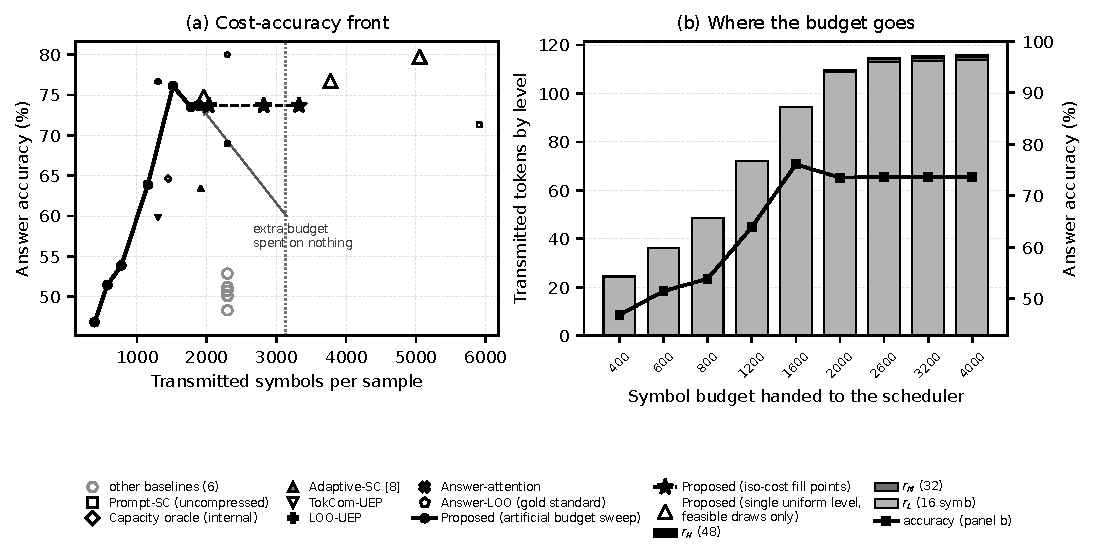
\includegraphics[width=0.78\textwidth]{images/fig_pareto.pdf}
\caption{等成本考核（主线配置端侧4B$\rightarrow$边侧8B，$15$~dB，3信道$\times$60样本$\times$3种子）。(a)实线为本文方法在人工预算$400$--$4000$下形成的精度--实际开销前沿，星号为填充至容量预言机、Adaptive-SC和词表类方法实际开销的等成本点，空心三角为全报告统一保护级端点（三档可行观测占比分别为$88\%$、$57\%$与$13\%$）。(b)授权预算、实际使用符号数（左轴）与精度（右轴）；实际开销在约$1900$个符号处饱和，继续增加预算不再改善精度。}
\label{fig:pareto}
\end{figure*}

图~\ref{fig:pareto}表明三点。（i）\textbf{额外预算不被使用}。给定预算由$2000$增至$4000$个符号时，实际开销只由$1774$增至$1898$个符号，精度在$73.5\%$与$73.7\%$之间波动（差异在置信区间内），说明该工作点增加预算无益。（ii）\textbf{强制等成本不改变任何逐题判定}。把开销按效用密度抬升至容量预言机、Adaptive-SC与词表类方法的实际水平（$2031$、$2817$与$3324$个符号）后三者精度同为$73.7\%$，与本文方法实际工作点（$3134$个符号，$73.7\%$）的配对检验均为$0{:}0$，即多花资源只用于提升保护等级；而$15$~dB下三档保护级的条件解码概率几乎相同（均受$5\%$丢包支配），故不带来任何精度增益。（iii）\textbf{成本过低才会损失精度}。预算下压至$800$、$600$与$400$个符号时精度依次降至$53.9\%$、$51.5\%$与$46.9\%$，真实拐点在$1200$至$1600$个符号之间。

上述结论可由式~\eqref{eq:expected_utility}解释。在$15$~dB下$q_{iH}\approx q_{iM}\approx q_{iL}=0.95$，提高保护等级只增加$r_{i\ell}^{(k)}$而不改变$z_{i,\tau}^{(k)}$，故额外预算无法转化为效用增益，此时决定性能的是被调度Token的覆盖范围而非单Token可靠性。

需要说明的是，全报告统一保护级的端点在某些工作点上看似更高（$15$~dB下$r_L$、$r_M$与$r_H$分别达$74.8\%$、$76.7\%$与$79.7\%$），但它们仅在整份报告恰好装得进可靠预算的观测上可行（分别占$88.1\%$、$56.5\%$与$12.8\%$），排除了深衰落观测；在同一可行子集上重算，本文方法的解与三者的精度完全相同（$74.8\%$、$76.7\%$与$79.7\%$对同值），逐格判定$100\%$一致，故差异来自样本子集而非策略优劣。

\subsection{信道适应性与多终端调度}
\label{sec:exp-scan}

\textbf{时变信道适应性。}
表~\ref{tab:main}覆盖$0$与$15$~dB两个工作点；本实验进一步将信号强度扩展为五点（$0$--$20$~dB），并对带宽（$0.25$--$2$~MHz）与CSI误差（$\sigma_e^2\in\{0.01,0.05,0.10\}$）做四档与三档扫描，结果见图~\ref{fig:snr}与图~\ref{fig:budgetcsi}。

\begin{figure}[t]
\centering
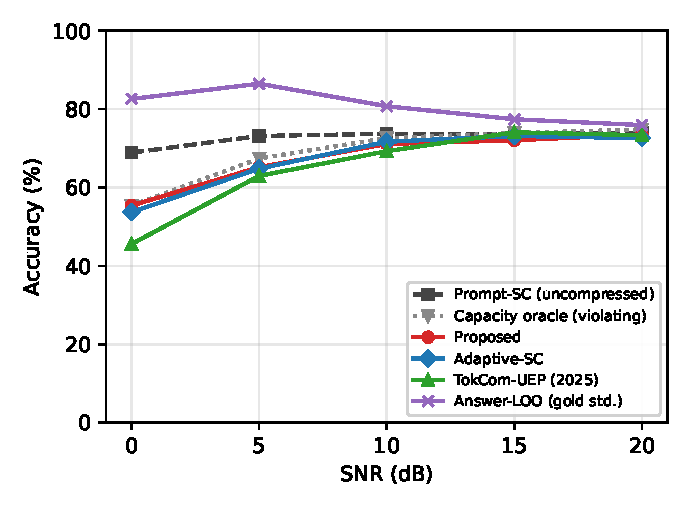
\includegraphics[width=\columnwidth]{images/fig_snr_sweep.pdf}
\caption{信号强度五点扫描（端侧4B$\rightarrow$边侧8B，公平接收端协议，衰落信道均值）。}
\label{fig:snr}
\end{figure}

\begin{figure*}[t]
\centering
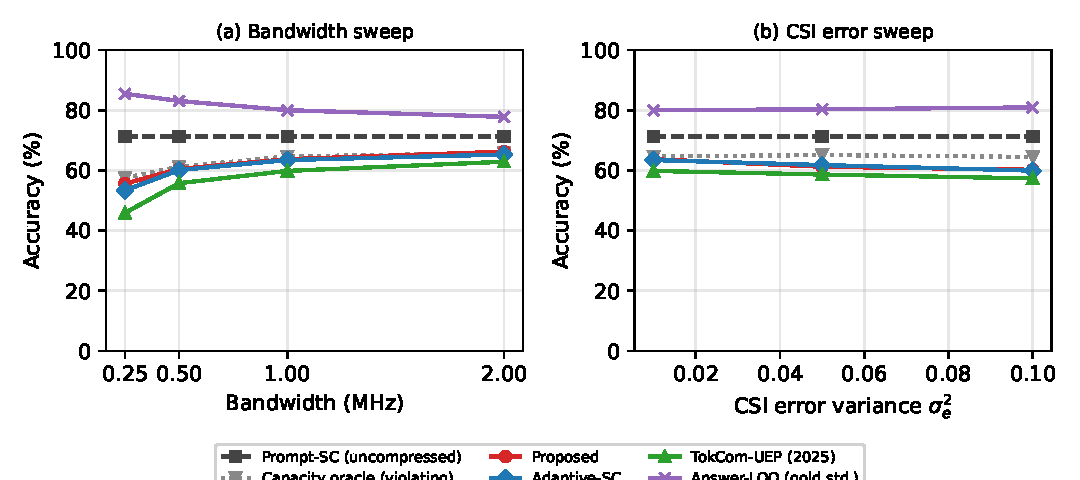
\includegraphics[width=0.72\textwidth]{images/fig_budget_csi.pdf}
\caption{带宽四档扫描（a）与CSI误差三档扫描（b）（配置同图~\ref{fig:snr}）。}
\label{fig:budgetcsi}
\end{figure*}

在\textbf{信号强度}维度，所提方法的累积精度（AUBC，按SNR梯形积分）为$68.2$，与Adaptive-SC（$68.2$）持平，高于TokCom-UEP（$66.4$），但所提方法的符号开销在中高信噪比上显著更低（$15$~dB时$1898$对$3134$、$20$~dB时$2047$对$4408$，分别节省$39\%$与$54\%$；$0$~dB处两者均顶满可靠预算，开销$706$对$700$）。$20$~dB时所提方法（$73.5\%$）与未压缩参考（$73.9\%$）无显著差异，此时擦除仅约$5\%$，瓶颈由信道转向报告与预算的匹配。在\textbf{带宽}维度（图~\ref{fig:budgetcsi}a），所提方法在四档上均不低于Adaptive-SC（$55.6\%$对$53.3\%$、$60.5\%$对$60.1\%$、$63.7\%$对$63.4\%$、$66.2\%$对$65.3\%$），且带宽越松符号节省越大（$2$~MHz下节省$45\%$）。在\textbf{CSI误差}维度（图~\ref{fig:budgetcsi}b），$\sigma_e^2$由$0.01$增至$0.10$时所提方法下降$3.5$个百分点（$63.7\%$至$60.2\%$），而不使用CSI的未压缩参考保持不变；预算违约率在三档分别为$0.2\%$、$1.1\%$与$1.2\%$，始终远低于目标$\varepsilon_{\mathrm{out}}=0.05$。

\textbf{多终端比例公平调度。}
\label{sec:exp-e}

表~\ref{tab:multiterminal}以$K=10$为例给出比例公平权重$\vartheta$扫描的结果（$15$~dB）。

\begin{table}[t]
\centering
\caption{多终端比例公平前沿（$K=10$，$15$~dB，准确率型的Jain指数在$0/1$向量上恒等于均值，故以\textbf{带宽}Jain指数衡量资源公平性）}
\label{tab:multiterminal}
\renewcommand{\arraystretch}{1.05}
\begin{tabular}{cccc}
\hline
$\vartheta$ & 平均精度(\%) & 带宽Jain指数 & 平均选中Token数\\
\hline
$0$ & 8.3 & 0.100 & 12.7\\
$0.01$ & 33.3 & 0.903 & 25.8\\
$0.05$ & 28.3 & 0.996 & 23.5\\
$0.1$ & 31.7 & 0.999 & 23.1\\
$1$ & 33.3 & 1.000 & 22.9\\
$10^{9}$ & 33.3 & 1.000 & 22.8\\
\hline
\end{tabular}
\end{table}

由表~\ref{tab:multiterminal}可见，$\vartheta=0$（式~\eqref{eq:joint_optimization}中仅保留任务效用项）会把全部带宽集中到边际语义价值最高的终端，平均精度仅$8.3\%$、带宽Jain指数$0.100$。引入很小的比例公平正则（$\vartheta=0.01$至$0.05$）后Jain指数即跃升至$0.903$至$0.996$，而平均精度不降反升（$28.3\%$至$33.3\%$），$\vartheta\geq0.1$后进入平台。该现象与第~\ref{sec:optimization}节的分析一致。当$\vartheta>0$时对数正则项使外层目标在带宽单纯形上严格凹，式~\eqref{eq:bandwidth_kkt}不仅必要而且充分，解唯一且稳定；$\vartheta=0$时该式退化为次梯度条件，对应不稳定的角点解。$K\in\{4,20\}$时规律相同，公平性均在$\vartheta\approx0.05$附近接近饱和。

\subsection{核心机制与部署验证}
\label{sec:exp-f}

\textbf{核心机制与理论条件。}
\label{sec:exp-d}
本实验集中核验可靠容量、集合耦合和期望效用形式三个核心设计。首先，四组代表条件下的实测Token擦除率与理论条件中断概率偏差均小于$1$个百分点：Rayleigh/$0$~dB为$27.5\%$对$27.9\%$，Rician/$0$~dB为$13.6\%$对$13.6\%$，频率选择性/$0$~dB为$26.6\%$对约$27\%$，Rayleigh/$15$~dB为$5.3\%$对$5.8\%$。所提方法实测中断率为$0.057$，较$0.05$目标高$0.7$个百分点，表明离散保护码本仍需更细粒度校准；直接代入估计CSI的容量预言机则有$51.1\%$的运行超出真实可用容量。

其次，联合删除前$25\%$与$50\%$的Token时，实测NLL增量与单Token边际增益之和的比值中位数分别为$0.098$与$0.087$，说明独立可加分数不能准确描述集合删除损失。全部$150$个样本均满足命题~\ref{prop:coupled_approx}要求的$\kappa_k<1$，其中位数为$0.194$、最大值为$0.439$，相应最坏情形近似下界不低于$[2(1+0.439)]^{-1}\approx0.347$。最后，将式~\eqref{eq:expected_utility}中的$q_{i\ell,\tau}^{(k)}$替换为$q^\gamma$后，$\gamma\in\{0,0.25,0.5\}$在开发集与测试集上均不优于$\gamma=1$；例如表现最好的$\gamma=0.25$在测试集上为$58.1\%$，而线性期望效用为$59.1\%$。因此正文采用的集合耦合和线性可靠性加权均得到实验支持。

\textbf{计算开销与部署限制。}
\label{sec:exp-lat}

任务响应时间从车辆获得图像与问题开始，到RSU输出答案结束。串行实现的阶段分解为
\begin{equation}
\begin{split}
T_{\mathrm{task}}={}&T_{\mathrm{report}}+T_{\mathrm{score}}
+T_{\mathrm{ctrl}}+T_{\mathrm{alloc}}\\
&+T_{\mathrm{select}}+T_{\mathrm{codec}}
+T_{\mathrm{UL}}+T_{\mathrm{infer}}.
\end{split}
\label{eq:task_latency}
\end{equation}
各项依次表示报告生成、语用评分、控制与窗口等待、RSU带宽分配、Token选择、载荷编解码、数据上行与接收端推理。总时延按逐样本时间线统计，父阶段与子阶段不重复相加，也不相加各阶段分位数。$T_s=1$~ms为获授权的数据窗口，不包含发送前计算。感知触发和答案回传位于上述计时边界之外。

阶段开销评估采用端侧4B$\rightarrow$边侧8B配置，bf16、batch size为1。计时机为单机双卡工作站：$2\times$NVIDIA GeForce RTX 3090（各$24$~GB，驱动版本$535.261.03$，计算能力$8.6$），端侧4B置于0号卡、边侧8B置于1号卡；CPU为Intel Core i9-12900K（$24$线程），内存$125$~GB；软件环境为Ubuntu（Linux 5.15.0-139）、Python 3.10.20、PyTorch 2.5.1+cu121（CUDA 12.1、cuDNN 9.1.0）与Transformers 4.57.6。在$0$与$15$~dB下分别使用固定信道实例（逐样本标识为4242加样本序号）与$30$个样本，每样本预热$5$次后重复$3$次；各方法在样本内的执行顺序随机化。\textbf{本文所有表格使用同一聚合规则：先把同一输入的重复观测归并为该输入的中位数，再对$30$个输入统计P50/P95与均值}（正确率例外，取全部记录的均值而非逐次$0/1$的中位数）；P95的秩取$\lceil0.95n\rceil$，等价于$30$个输入中的最大值。报告长度中位数在两档均为$121$个Token，本文方法在$15$~dB与$0$~dB下分别选中$118$与$18$个Token、交付$111$与$17$个。受限于$30$个输入的样本量，P95为小样本估计，比较$1$~ms量级差异时以逐样本差值为准。两档结果描述给定交付文本长度下的计算开销，不代表跨衰落总体统计。

\begin{table*}[t]
\centering
\caption{本文方法的阶段计算开销（ms，P50/P95；30样本，每样本3次重复；两档为固定信道实例）}
\label{tab:latency_stages}
\renewcommand{\arraystretch}{1.05}
\begin{tabular}{lccp{0.45\textwidth}}
\hline
阶段 & $15$~dB & $0$~dB & 计时范围\\
\hline
报告生成总计 & 2331.10/2866.23 & 2331.58/2870.78 & 图像处理、文本生成与解码；视觉塔为诊断测量不另加\\
\quad 报告输入组装 & 6.87/7.72 & 6.97/7.89 & 含图像的多模态输入组装与设备搬运\\
\quad 报告文本生成 & 2315.08/2853.36 & 2323.58/2858.04 & 自回归生成（子项，不重复计入总计）\\
\quad 报告解码与释放 & 6.89/7.43 & 6.94/7.40 & 文本解码、删除中间张量与释放缓存\\
语用评分总计 & 325.74/350.76 & 329.67/355.31 & 输入准备、前向、聚合、反向、耦合与结果处理\\
\quad 评分输入准备 & 12.62/13.08 & 12.58/13.52 & 两次多模态输入处理与报告区间定位\\
\quad 提示搬运与标签构造 & 0.05/0.06 & 0.05/0.06 & 标识与掩码搬运、答案标签拼接\\
\quad 教师强制前向 & 113.78/119.23 & 114.98/119.64 & 输出注意力，包含视觉Token\\
\quad 梯度与损失处理 & 104.75/110.32 & 106.60/112.16 & 包含掩码前向、损失构造与反向传播\\
\quad 答案NLL同步 & 0.02/0.02 & 0.02/0.02 & 取回标量损失至CPU\\
\quad 结果序列化（批量搬运） & 0.17/0.40 & 0.17/0.39 & 一次性搬回后转换，正式路径\\
\quad （对照）逐元素序列化 & 2.04/2.53 & 2.06/2.49 & $N^2$次标量搬运，诊断项，不计入总计\\
\quad 缓存释放 & 90.94/106.88 & 91.62/107.65 & 删除中间张量与显存分配器回收\\
\quad （父-子残差） & 1.15/1.44 & 1.10/1.30 & 父项减子项之和，仅作校验\\
Token选择与保护调度 & 1.90/3.06 & 1.93/2.60 & 基础LP、极点舍入与最多8次局部改进\\
RSU带宽协调 & 1.16/1.18 & 1.17/1.19 & $K=10$，CPU语义价格处理与带宽分配\\
接收端输入处理 & 0.48/0.64 & 0.39/0.52 & 模板构造、分词与设备搬运\\
接收端单次前向 & 50.04/56.14 & 26.37/55.37 & 获取末位logits\\
接收端答案读出 & 0.07/0.09 & 0.07/0.08 & 候选字母logits批量搬至CPU后取最大值\\
\quad（对照）逐字母同步读出 & 38.69/43.17 & 20.01/43.99 & 每字母一次标量搬运，诊断项，不进入正式路径\\
\hline
\end{tabular}
\end{table*}

表~\ref{tab:latency_stages}显示，已测阶段中报告生成约为$2.33$~s（其中文本生成本身占$2.32$~s），当前语用评分实现约为$0.33$~s，而Token选择与保护调度约为$1.9$~ms。评分成本中约$91$~ms来自\texttt{empty\_cache}式的显存分配器回收，属当前实现开销而非模型计算，可通过复用分配器或延迟释放消除，故不计入方法的必要计算。结果序列化原按元素逐个回传（$N^2$次标量搬运，$2.04$~ms），改为一次性批量搬回后降至$0.17$~ms，两档一致；逐元素实现保留为对照且不计入总计。补齐报告组装、解码与提示搬运等插桩后，逐次父子残差P50/P95在两档降至$1.15/1.44$~ms与$1.10/1.30$~ms，即$15$个阶段边界同步开销的量级；残差仅用于校验，不作为额外阶段加入总时延，也不以分位数相减的方式计算。阶段耗时不直接证明每个$1$~ms窗口均能完成调度，该问题在本节末的资源映射中单独讨论。

\begin{table}[t]
\centering
\caption{当前实现的Token选择与保护处理耗时（ms，P50/P95；不包含报告生成和重要性评分）}
\label{tab:latency_selection}
\renewcommand{\arraystretch}{1.05}
\begin{tabular}{lcc}
\hline
选择器 & $15$~dB & $0$~dB\\
\hline
本文方法 & 1.90/3.06 & 1.93/2.60\\
Adaptive-SC（内部变体） & 0.91/1.08 & 0.54/0.92\\
TokCom-UEP & 1.79/2.51 & 1.79/2.34\\
未压缩参考 & 0.32/0.36 & 0.32/0.38\\
\hline
\end{tabular}
\end{table}

表~\ref{tab:latency_selection}仅比较选择器处理成本，其中\textbf{Adaptive-SC为内部变体}：其选级规则直接消费本文的三维语用评分（数据中以\texttt{baseline\_role}字段标注），并非原基线的独立实现，故不能把它的耗时记为原基线的必要计算。TokCom-UEP的重要性来自外部模型，这里只计入其\textbf{缓存读取与归一化}（$0.014$~ms），其离线生成成本未测、不默认零。因此不能依据选择器耗时推断各方法的完整必要计算成本或任务响应排名。

\textbf{接收端读出。}在相同输入与交付文本下，边侧8B比较单次前向判别式读出与自回归字母输出。每档对\textbf{每个方法}各取$30$个样本、重复$3$次，即每方法$90$条、四方法共$360$条方法--样本观测；方法间共享同一批源样本，故这些观测不视为$360$个独立场景。

\begin{table*}[t]
\centering
\small
\caption{边侧8B读出对照（ms，P50/P95；每个方法每档$30$个输入、每输入重复$3$次，先取每输入中位再对$30$个输入统计；四种方法共享同一交付文本）}
\label{tab:latency_readout}
\renewcommand{\arraystretch}{1.05}
\begin{tabular}{lcccccc}
\hline
 & \multicolumn{2}{c}{$15$~dB} & \multicolumn{2}{c}{$0$~dB} & 输出 & 精度 (\%)\\
 & 判别式 & 自回归 & 判别式 & 自回归 & 长度 & $15$/$0$~dB\\
\hline
本文方法 & 50.1/56.2 & 114.0/125.9 & 26.4/55.4 & 76.2/132.0 & 1 & 73.3/60.0\\
Adaptive-SC & 50.1/61.7 & 114.6/132.4 & 26.3/56.0 & 78.1/127.9 & 1 & 73.3/60.0\\
TokCom-UEP & 50.2/60.9 & 114.6/130.9 & 26.6/51.2 & 74.4/126.0 & 1 & 73.3/53.3\\
未压缩参考 & 50.4/65.4 & 114.4/148.0 & 54.4/65.1 & 116.8/151.0 & 1 & 76.7/70.0\\
\hline
\multicolumn{7}{p{0.95\textwidth}}{答案一致率在两档、四个方法上均为$100\%$（$360/360$）；自回归实际早停于$1$个Token，生成上限$24$未触及。若改为对全部$90$条观测直接统计，P50变化不超过$0.3$~ms，P95变化可达$10$~ms}\\
\hline
\end{tabular}
\end{table*}

表~\ref{tab:latency_readout}按方法分别报告，配对名单已均衡：每个方法在每档恰好为$30$个输入$\times3$次重复$=90$条观测，四种方法合计$360$条，且方法间共享同一批源样本，故不视为$360$个独立场景。两种读出在同一交付文本上运行，答案一致率在两档、四个方法上均为$100\%$，即改用判别式读出\emph{不改变任何一条交付答案}；表中逐方法精度与表~\ref{tab:latency_baselines}的同条件精度逐一对应。判别式列计入该方法的接收端输入处理、单次前向与批量读出，故随交付长度变化：$0$~dB下未压缩参考交付$111$个Token，其$54.4$~ms显著高于其余方法的$26.3$--$26.6$~ms，而$15$~dB下四者接近$50$~ms，因此不能与表~\ref{tab:latency_stages}中单一方法的前向分位数拼接。自回归输出在两档均实际早停于$1$个Token（生成上限$24$未触及），该列反映的是首Token判定路径的代价，而非上限长度下的代价；候选logits采用一次性批量搬运，逐字母同步搬运仅作实现诊断，不进入正式读出路径。

\textbf{完整响应与资源映射。}本文固定的资源口径为：每Token信息量$16$~bit，保护级$H/M/L$的编码开销为$48/32/16$个等效比特（对应码率$1/3,1/2,1$），每符号承载$1$个编码比特，故信道使用数等于编码比特数；单个数据窗口（$T_s=1$~ms、$B=1$~MHz）可承载$1000$个符号，即$1000$个编码比特。式~\eqref{eq:reliable_capacity}给出的$C_\tau$是\emph{等效比特预算}（$15$~dB与$0$~dB下分别为$4036$与$574$），其中$15$~dB的取值约为单窗口物理容量的$4.04$倍，即它对应约$4$个授权窗口的累计容量，不能当作单窗口的物理装载上限。因此本文以\textbf{窗口数}为物理资源轴，逐样本按$\lceil$编码比特$/1000\rceil$计算并报告其中位与均值，不由中位开销倒推；$0$~dB下可靠容量本身低于单窗口容量（$574<1000$），物理上限未绑定。按此口径，未压缩参考的编码开销为$5808$个等效比特（$6.0$个窗口中位、最多$9$个），在$15$~dB与$0$~dB下分别有$83.3\%$与$100\%$的样本超出该实例的等效预算，故只能作为\textbf{超预算参考}，其额外窗口必须计入资源与比较条件。控制等待、载荷打包与编解码，以及TokCom外部信号的离线获取仍未测量，不能默认其耗时为零；含未测项的响应时间仅作部分估计，不用于完整链路排名。表~\ref{tab:latency_baselines}汇总同条件结果。

\begin{table*}[t]
\centering
\caption{同条件精度、物理资源与必要计算成本（$30$样本$\times3$重复；资源成本为编码比特；计算为逐样本中位数后再取跨样本中位数，单位ms）}
\label{tab:latency_baselines}
\renewcommand{\arraystretch}{1.05}
\small
\setlength{\tabcolsep}{4pt}
\begin{tabular}{llrrrrrrrr}
\hline
实例 & 方法 & 精度 & 信息比特 & 资源成本 & 窗口数 & 超预算 & 场景1 & 场景2 & 场景3\\
 & & (\%) & & (编码比特) & 中位(均值) & (\%) & 含报告 & 缓存报告 & 全缓存\\
\hline
$15$~dB & 本文方法 & 73.3 & 1880 & 1952 & 2.0 (2.33) & 0.0 & 2710.5 & 379.4 & 53.7\\
$15$~dB & Adaptive-SC（内部变体） & 73.3 & 1880 & 2984 & 3.5 (3.50) & 0.0 & 2709.6 & 378.5 & 52.7\\
$15$~dB & TokCom-UEP & 73.3 & 1880 & 1952 & 2.0 (2.33) & 0.0 & 2384.8 & 53.7 & 53.7\\
$15$~dB & 未压缩参考（超预算） & 76.7 & 1936 & 5808 & 6.0 (6.17) & 83.3 & 2383.4 & 52.3 & 52.3\\
$0$~dB & 本文方法 & 60.0 & 280 & 568 & 1.0 (1.27) & 0.0 & 2691.3 & 359.7 & 30.1\\
$0$~dB & Adaptive-SC（内部变体） & 60.0 & 280 & 560 & 1.0 (1.27) & 0.0 & 2689.6 & 358.1 & 28.4\\
$0$~dB & TokCom-UEP & 53.3 & 280 & 568 & 1.0 (1.27) & 0.0 & 2361.7 & 30.1 & 30.1\\
$0$~dB & 未压缩参考（超预算） & 70.0 & 1936 & 5808 & 1.0 (1.27) & 100.0 & 2388.0 & 56.5 & 56.5\\
\hline
\multicolumn{10}{p{0.95\textwidth}}{单窗口物理容量$1000$个编码比特；预算等价窗口为$15$~dB的$4.04$与$0$~dB的$1.00$。场景1--3依次为报告未缓存、报告缓存但评分重算、报告与评分均缓存；端口上行固定为$1$个时隙（模拟）}\\
\hline
\end{tabular}
\end{table*}

\noindent\textit{[待补充：含控制等待与编解码的完整时间线、按真实Token长度的评分与局部搜索扫描、$K=4/10/20$协调测试，以及覆盖CSI老化与窗口等待的验证。]}

已有结果支持：报告生成与语用评分具有显著计算成本，Token选择本身为毫秒量级；在同一批样本与信道实例下，本文方法与Adaptive-SC内部变体精度相同（$15$~dB均为$73.3\%$）而编码资源成本低$34.6\%$（$1952$对$2984$个等效比特）、窗口数$2.0$对$3.5$，$0$~dB下则在完全相同的$568$个等效比特上比TokCom-UEP高$6.7$个百分点；读出改为判别式后答案逐条不变。需要强调的是，\textbf{各方法的完整任务时延并不并列}：场景2下本文方法与Adaptive-SC的语用评分成本约$0.36$~s，比不消费评分的TokCom-UEP与未压缩参考高约$0.33$~s，而TokCom-UEP的外部信号离线成本尚未计入，故当前响应时间只能作为部分时间估计，不支持完整链路排名。本文的通信资源效率收益亦不等同于任务响应时间收益。

\balance
\section{结论}
\label{sec:conclusion}

本文面向时变多终端信道，将生成式语义通信由提示序列级传输推进到Token级语用感知选择。所提出的统一语用度量融合因果自注意力结构重要度、语义方向一致性和删除感知梯度敏感度，集合相关的语义耦合模型只评价实际成功接收的上下文；可靠容量与条件解码概率进一步把Token效用、编码保护和不完美CSI联系起来。由此形成的二次多选择背包问题先经拉格朗日松弛与极点舍入获得可行解，再由耦合感知局部搜索改进；在线语义价格则实现由KKT条件导出的比例公平带宽分配。理论分析将端到端性能差距分解为离散优化、语义代理、模型失配和信道中断四类误差，并建立Token保留率、可靠等效比特率与VQA错误概率上界之间的联系。

现有实验从任务性能、信道适应性、多终端公平性和核心机制验证了上述设计，阶段计算开销已作测量，完整任务时延仍待验证。所提方法在可部署方法中取得最高资源效率：相对精度最强基线提升$47.9\%$，在精度统计不可区分时减少约$32\%$的传输符号；未经筛选的全部$150$个样本亦保持相同结论。其优势在不同SNR、带宽和CSI误差下保持稳定，比例公平正则可避免多终端带宽分配退化为角点解。可靠容量校准、集合交互和线性可靠性加权的核验支持了关键建模选择，但$0.057$的实测中断率仍略高于$0.05$目标。阶段测量显示，报告生成与语用评分具有显著计算开销（其中约$91$~ms属显存分配器回收等实现开销），Token调度本身为毫秒量级；同条件对照显示，本文方法与Adaptive-SC内部变体精度相同而编码资源成本低$34.6\%$、窗口数更少，$0$~dB下在相同资源上优于TokCom-UEP，8B读出改为判别式后答案逐条不变。完整任务响应仍受未测的控制等待、编解码与外部信号离线成本限制，故不作链路时延排名。未来工作将细化离散保护码本、降低报告生成与推理时延，并扩展到干扰耦合的多通信对调度。

\bibliographystyle{IEEEtran}
\bibliography{references}

\end{document}
